%%%%%%%%%%%%%%%%%%%%%%%%%%%%%%%%%%%%%%%%%%%%%%%%%%%%%%%%%%%%%%%%%%%%%%%%%%%%%%%
%                         File: osa-revtex4-1.tex                             %
%                        Date: April 15, 2013                                 %
%                                                                             %
%                              BETA VERSION!                                  %
%                   JOSA A, JOSA B, Applied Optics, Optics Letters            %
%                                                                             %
%            This file requires the substyle file osajnl4-1.rtx,              %
%                   running under REVTeX 4.1 and LaTeX 2e                     %
%                                                                             %
%                   USE THE FOLLOWING REVTeX 4-1 OPTIONS:                     %
% \documentclass[osajnl,twocolumn,showpacs,superscriptaddress,10pt]{revtex4-1}%
%                    %% Use 11pt for Applied Optics                           %
%                                                                             %
%               (c) 2013 The Optical Society of America                       %
%                                                                             %
%%%%%%%%%%%%%%%%%%%%%%%%%%%%%%%%%%%%%%%%%%%%%%%%%%%%%%%%%%%%%%%%%%%%%%%%%%%%%%%

\documentclass[osajnl,twocolumn,showpacs,superscriptaddress,10pt]{revtex4-1} %% use 10pt for Applied Optics
%%\documentclass[osajnl,preprint,showpacs,superscriptaddress,12pt]{revtex4-1} %% use 12pt for preprint option
\usepackage{amsmath,amssymb,graphicx,float,enumerate}
\usepackage[cache=false]{minted}
\usepackage[utf8]{inputenc}
\graphicspath{ {../images/} }

\usepackage[colorlinks = true,
            linkcolor = black,
            urlcolor  = blue,
            citecolor = black,
            anchorcolor = blue]{hyperref}

\usepackage{silence}
\WarningFilter{revtex4-1}{Repair the float}

\begin{document}

\title{Redes y Comunicaciones}

\author{Ulises Jeremias Cornejo Fandos}
\affiliation{13566/7, Licenciatura en Informatica, Facultad de Informatica, UNLP}

\author{Federico Ramón Gasquez}
\affiliation{13598/6, Licenciatura en Informatica, Facultad de Informatica, UNLP}

\author{Lihuel Pablo Amoroso}
\affiliation{13497/2, Analista Programador Universitario, Facultad de Informatica, UNLP}

%%\begin{abstract}
%%\end{abstract}

\maketitle %% required

\onecolumngrid

\section{Introducción}

\textit{En la máquina virtual, instale el paquete radvd (sudo apt update; sudo apt install -y radvd).} \\

Utilizando la topología enlace-Ipv6.imn:

\begin{itemize}
    \item Analice las direcciones IPv6 de PC-A y PC-B:
    
    \begin{itemize}
        \item ¿Cuántas direcciones IP tiene cada interfaz?
        \item ¿Cuáles son?
        \item ¿Qué alcance tiene cada una de ellas?
    \end{itemize}
\end{itemize}

Analizando este aspecto de la topología observamos que ninguna de las interfaces
dispone de una IP asignada a simple vista. Sin embargo, luego de iniciar la topología,
se ejecuta el comando \textit{ifconfig} sobre cada uno de los hosts
viendo así las IPs asignadas a cada uno. En ambos casos se observan dos IPs asignadas, una de alcance local al enlace y otra de alcance global. \\

Concretamente las IPs asignadas, con su correspondiente alcance, son:

\begin{itemize}
    \item \textbf{PC-A}
    
    \begin{itemize}
        \item inet6 addr: \textbf{fe80::200:ff:feaa:1/64} Scope: \textbf{Link}
        \item inet6 addr: \textbf{2001::200:ff:feaa:1/64} Scope: \textbf{Global}
    \end{itemize}

    \item \textbf{PC-B}
    
    \begin{itemize}
        \item inet6 addr: \textbf{fe80::200:ff:feaa:0/64} Scope: \textbf{Link}
        \item inet6 addr: \textbf{2001::200:ff:feaa:0/64} Scope: \textbf{Global}
    \end{itemize}
\end{itemize}

\section{Router advertisement - Análisis}

En PC-A, desconecte y conecte la interfaz mientras captura tráfico. \\

Analice los mensajes “Router Solicitation” y “Router advertisement”. \\

En la figura (\ref{image:router-solicitation-advertisement}) se observa la captura de paquetes durante 
la conexión de la interfaz eth0 en PC-A. \\

Los mensajes \textit{Router Advertisement} y \textit{Router Solicitationes} permiten que un nodo en un enlace descubra los routers 
en el mismo enlace. Cada interfaz de enrutador configurada en un enlace envía un mensaje de Router Advertisement, 
que tiene un valor de 134 en el campo \textit{Type} del encabezado del paquete ICMP, periódicamente a la dirección 
de multicast local de enlace de todos los nodos (\textit{FF02::1}). \\

Una interfaz de enrutador configurada también puede enviar un mensaje de Router Advertisement en respuesta a un mensaje 
de Router Solicitation desde un nodo en el mismo enlace. Este mensaje se envía a la dirección IPv6 de unicast del nodo 
que envió el mensaje de Router Solicitation.

Al iniciar el sistema, un host en un enlace envía un mensaje de Router Solicitation a la dirección de multicast de todos 
los routers (\textit{FF01}). El envío de un mensaje de Router Solicitation, que tiene un valor de 133 en el 
campo \textit{Type} del encabezado del paquete ICMP, permite al host configurar automáticamente su dirección IPv6 
inmediatamente en lugar de esperar el próximo mensaje periódico de anuncio del enrutador. \\

Debido a que un host en el inicio del sistema generalmente no tiene una dirección IPv6 de unicast, la dirección de origen 
en el mensaje de solicitud del enrutador suele ser la dirección IPv6 no especificada (0:0:0:0:0:0:0:0). 
Si el host tiene una dirección IPv6 de unicast, la dirección de origen es la dirección IPv6 de unicast 
de la interfaz del host que envía el mensaje de Router Solicitation. \\

\begin{figure}[H]
    \centering
    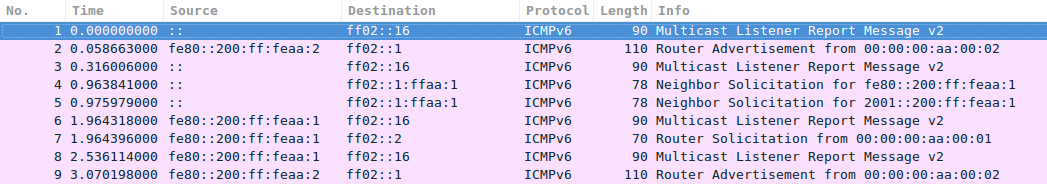
\includegraphics[width=0.95\textwidth]{router-solicitation-advertisement.png}
    \caption{Captura de paquetes durante la conexión de la interfaz eth0 en PC-A.}
    \label{image:router-solicitation-advertisement}
\end{figure}

\section{Router solicitation}

\begin{itemize}
    \item ¿Cuál es el tipo y el código del mensaje?
    
    

    \item ¿Cuál es la MAC origen y la MAC destino?
    
    \begin{itemize}
        \item ¿Qué tipo de MAC es la MAC destino?
    \end{itemize}

    \item ¿Cuál es la IP origen y la IP destino?
    
    \begin{itemize}
        \item ¿Qué tipo de dirección es la IP origen y qué tipo de dirección es la IP destino?
    \end{itemize}

    \item ¿Qué datos puede destacar del mensaje ICMP?
\end{itemize}

\section{Router advertisement}

\begin{itemize}
    \item ¿Cuál es el tipo y el código del mensaje?
    \item ¿Cuál es la MAC origen y la MAC destino?
    
    \begin{itemize}
        \item ¿Qué tipo de MAC es la MAC destino?
    \end{itemize}
    
    \item ¿Cuál es la IP origen y la IP destino?
    
    \begin{itemize}
        \item ¿Qué tipo de dirección es la IP origen y qué tipo de dirección es la IP destino?
    \end{itemize}
    
    \item ¿Qué datos puede destacar del mensaje ICMP? ¿Cuál es prefijo que se anuncia?
\end{itemize}

\section{Análisis de rutas}

Visualice la tabla de rutas de IPv6:

\begin{itemize}
    \item ¿Cuál es el default GW de PC-A? ¿Qué alcance tiene dicha dirección?
\end{itemize}

Verifique conectividad entre PC-A y “SERVER”.

\section{Neighbor discovery - Análisis}

\textit{Desde PC-A haga un ping a la IPv6 global de PC-B mientras captura tráfico ICMPv6 en
PC-B. Analice los mensajes “Neighbor Solicitation” y “Neighbor Advertisement”.}

\section{Neighbor solicitation}

\begin{itemize}
    \item ¿Cuál es el tipo y el código del mensaje?
    \item ¿Cuál es la MAC origen y la MAC destino?
    
    \begin{itemize}
        \item ¿Qué tipo de MAC es la MAC destino?
    \end{itemize}
    
    \item ¿Cuál es la IP origen y la IP destino?
    
    \begin{itemize}
        \item ¿Qué tipo de IP es la IP destino?
    \end{itemize}
    
    \item ¿Qué datos puede destacar del mensaje ICMP?
\end{itemize}

\section{Neighbor Advertisement}

\begin{itemize}
    \item ¿Cuál es el tipo y el código del mensaje?
    \item ¿Cuál es la MAC origen y la MAC destino?
    
    \begin{itemize}
        \item ¿Qué tipo de MAC es la MAC destino?
    \end{itemize}
    
    \item ¿Cuál es la IP origen y la IP destino?
    
    \begin{itemize}
        \item ¿Qué tipo de IP es la IP destino?
    \end{itemize}
    
    \item ¿Qué datos puede destacar del mensaje ICMP?
\end{itemize}

\textit{Visualice la tabla de caché de NDP de PC-A utilizando las herramientas provistas por
iproute2.}

\end{document}
